\documentclass{beamer}
\usepackage{amsmath}
\usepackage{graphicx}
\usepackage{cite}
\usepackage{tikz}
\usepackage{amsmath}
\usepackage{graphicx}

\usepackage{tikzit}

\usetikzlibrary{arrows.meta,positioning}
\usetikzlibrary{shapes.multipart,matrix,positioning,arrows,arrows.meta}
\usefonttheme{serif}
\tikzstyle{black circle}=[fill=white, draw=black, shape=circle, tikzit shape=circle]
\tikzstyle{Arrow}=[->]

% Edge styles
\tikzstyle{new edge style 0}=[->]

\setbeamertemplate{footline}[frame number]{}
\setbeamertemplate{navigation symbols}{}

\usecolortheme{lily}
\setbeamercolor{block title}{bg=blue!20,fg=black}
\setbeamercolor{block body}{bg = blue!10, fg = black}
\setbeamertemplate{itemize item}[square]
\setbeamercolor{itemize item}{fg = cyan}
\setbeamercolor{enumerate item}{fg = cyan}

\usetheme{default}
\beamertemplatenavigationsymbolsempty
\setbeamercolor{titlelike}{fg=blue}
\setbeamertemplate{caption}{\insertcaption\par}

%Information to be included in the title page:
\title{Strain-space model for Sars-CoV-2}
\author{Peter C. Jentsch, PhD \inst{1,4} \and Finlay Maguire, PhD  \inst{3,5} \and Samira Mubareka, MD, FRCPC \inst{1,2}}
\institute{\inst{1} Sunnybrook Research Institute, Toronto, Canada  \and \inst{2} University of Toronto, Toronto, Canada \and \inst{3} Dalhousie University, Halifax, Canada \and \inst{4} Simon Fraser University, Burnaby, Canada \and \inst{5} Shared Hospital Laboratory, Toronto, Canada}
\date{\today}

\begin{document}
\setbeamertemplate{caption}{\insertcaption\par}
\frame{\titlepage}

\begin{frame}
    \begin{itemize}
        \item Infection spread is often modelled using compartmental models

        \item Represent subsets of a host population and rates of movement between them
    \end{itemize}

    \begin{figure}
        \centering
            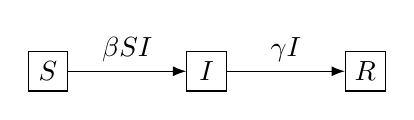
\begin{tikzpicture}[node distance=1.5cm, auto,
                >=Latex, 
                every node/.append style={align=center},
                int/.style={draw, minimum size=0.5cm}]
            
            \node [int] (S)             {$S$};
            \node [int, right=of S ] (I) {$I$};
            \node [int, right=of I] (R) {$R$};
            \path[->] (S) edge node {$ \beta S I$} (I);
            \path[->] (I) edge node {$\gamma I$} (R);
            \end{tikzpicture}
            \label{SIR_diagram}
    \end{figure}
    
\end{frame}

\begin{frame}
    \begin{columns}
        \begin{column}{0.6\textwidth}

            \begin{itemize}
                \item Multiple infections (e.g. competing VoCs) can be represented as more compartments
                \item Work on multiple infections is usually here due to lack of data, increasing complexity
            \end{itemize}
    
\end{column}


    \begin{column}{0.4\textwidth}

\begin{figure}[h!]
    \centering
    \includegraphics[width=\textwidth]{voc_model_diagram.png}
\label{model_structure}
\end{figure}
\end{column}
\end{columns}
% (e.g. \cite{Alizon_van_Baalen_2008, van_Baalen_Sabelis_1995, Lipsitch_Colijn_Cohen_Hanage_Fraser_2009, Nicoli_Ayabina_Trotter_Turner_Colijn_2015})
\end{frame}

\begin{frame}
    This only represents a tiny amount of the genomic data we have for Sars-CoV-2!
    \begin{figure}
        \includegraphics[width=0.5\textwidth]{phylogeny.png}
    \end{figure}
\end{frame}
\begin{frame}
    \begin{columns}
\begin{column}{\textwidth}
    \begin{figure}
        \includegraphics[width=0.6\textwidth]{gog_paper.png}
    \end{figure}
    \begin{figure}
        \includegraphics[width=0.6\textwidth]{gog_paper_2.png}
    \end{figure}
    % \begin{itemize}
    %     \item Can extend these models to a sequence of variants
    %     \item Assume each variant is indexed by $i$ 
    %     \item The dynamics at each variant $i$ are determined by a simple compartmental model
    % \end{itemize} 
    % \centering
    % \vspace{5cm}
    % \tiny{\cite{gogDynamicsSelectionManystrain2002}}
\end{column}
\end{columns}



\end{frame}
\begin{frame}
    \begin{columns}
        % \begin{column}{0.5\textwidth}
        %     \begin{itemize}
        %         \item Variants are related by a function $\sigma(i,j)$ that determines how much an infection by variant $i$ reduces probability of infection to variant $j$.
        %         \item A variant $i$ mutates to neighbouring indices $i+1, i-1$ proportional to the population of variant $i$
        %         \end{itemize}         
        % \end{column}
        \begin{column}{0.5\textwidth}
            \begin{figure}
                \includegraphics[width=\textwidth]{gog_fig.png}
            \end{figure}
        \end{column}
    \end{columns}
    \centering
    \vfill
    \tiny{\cite{gogDynamicsSelectionManystrain2002}}
\end{frame}
\begin{frame}
    \begin{columns}
        \begin{column}{0.5\textwidth}
            \begin{figure}
                \includegraphics[width=\textwidth]{gog_2d_a.png}
            \end{figure}        
        \end{column}
        \begin{column}{0.5\textwidth}
            \begin{figure}
                \includegraphics[width=\textwidth]{gog_2d_b.png}
            \end{figure}
        \end{column}
    \end{columns}
    \centering
    \vfill
    \tiny{\cite{gogDynamicsSelectionManystrain2002}}

\end{frame}

\begin{frame}{Antigenic cartography }

    \begin{columns}
        \begin{column}{0.5\textwidth}
            Technique developed to visualize the antigenic drift of influenza A (H3N2)
        \end{column}
        \begin{column}{0.4\textwidth}
        \begin{figure}
        \includegraphics[width=\textwidth]{smith_antigenic.png}    
        \end{figure}   
    \end{column}
    \end{columns}
    \centering
    \vfill
    \tiny{\cite{lapedesGeometryShapeSpace2001,smithMappingAntigenicGenetic2004}}
    % \begin{itemize}
    %     \item Practice of mapping out immune responses to related pathogens
    %     \item Distance between serums and pathogen is quantified, these points are visualized using multidimensional scaling (MDS)
% ,  usually as proportional reduction in serum viral titre hemaagglutinin assay
    % \end{itemize}
\end{frame}

\begin{frame}
    \begin{columns}
        \begin{column}{0.4\textwidth}
            \begin{figure}
                \includegraphics[width=1.4\textwidth]{mds_1.png}
                
            \end{figure}   
        \end{column}
        \begin{column}{0.01\textwidth}
            \huge{$\Longrightarrow$}
            
        \end{column}
        \begin{column}{0.4\textwidth}
            \begin{figure}
            \includegraphics[width=\textwidth]{mds_2.png}
            
        \end{figure}   
        \end{column}
    \end{columns}
    \centering
    \vfill
    \tiny{\cite{scikit-learn}}

\end{frame}

\begin{frame}
        \begin{figure}
        \includegraphics[width=\textwidth]{wilks.png}
    \end{figure}   
    \centering
    \vfill
    \tiny{\cite{wilksMappingSARSCoV2Antigenic2022}}
\end{frame}

\begin{frame}
    These results suggest that 2 dimensions might be an adequate approximation to the full space!
\end{frame}


\begin{frame}{Incorporating more data}
    \begin{itemize}
        \item A huge amount of genomic data is available
        % \item We have millions of samples and hundreds of thousands of unique genomes from random sampling alone
        \item Assign each sample to its closest lineage in the map from \cite{wilksMappingSARSCoV2Antigenic2022}
        \item Two methods to further differentiate genomes: homoplasic mutations or antibody binding
        % Distance between any two samples is determined by the distance between the respective closest lineage in Wilks, plus the SNP distance, where each SNP is weighted by how often it recurs in the global tree
    \end{itemize}
\end{frame}

\begin{frame}{Mutation homoplasy}
    \begin{figure}
        \includegraphics[width=\textwidth]{gene_freq.png}
    \end{figure}
\end{frame}
\begin{frame}{Antibody Binding map}
    \begin{figure}
        \includegraphics[width=\textwidth]{usa_multidimensional_scaling_binding.png}
    \end{figure}
\end{frame}

\begin{frame}{Homoplasic mutations map}
    \begin{figure}
        \includegraphics[width=\textwidth]{usa_multidimensional_scaling_snps.png}
    \end{figure}
\end{frame}



\begin{frame}{Evaluating the MDS approximation}
    \begin{figure}
        \includegraphics[width=\textwidth]{usa_mds_stress.png}
    \end{figure}
\end{frame}

    
\begin{frame}{}
    (animation of kernel approximation)
\end{frame}
\begin{frame}{Model parameters/variables}
    \begin{table}[h!]
        \begin{center}
        \begin{tabular}{c|p{8cm}}
                Symbol & Description \\
                \hline
                \hline
                $N$ & Size of variant grid \\
                $S_{ij}$ & Population susceptible to variant $(i,j) \in [0,N]^2$ \\
                $I_{ij}$ & Population infected by variant $(i,j) \in [0,N]^2$\\
                $R_{ij}$ & Recovered/Immune to variant $(i,j) \in [0,N]^2$\\
                $\sigma_{ijkl}$ & Probability that exposure to variant $(i,j)$ causes immunity \newline to variant $(k,l)$\\
                $\beta_{ij}$ & Transmission rate of variant $(i,j)$\\
                $v(t)$ & vaccination rate at time $t$\\
                $s(t)$ & stringency at $t$\\
                $\xi$ & Recovery rate of all strains \\
                $\gamma$ & Rate of immunity loss of all strains \\
        \end{tabular}
        \caption{Table of symbols for Model 2}
    
        \label{variables_2}
        \end{center}
    \end{table}
\end{frame}
\begin{frame}{Model Equations}
    \small
    \begin{equation}
        \frac{S_{ij}}{dt} = -\sum_{kl} s(t) \beta_{kl} \sigma_{ijkl} S_{ij} I_{kl} + \gamma R_{ij} - V(t)S  \label{Seqn}
    \end{equation}
    \begin{equation}
        \frac{ I_{ij}(t)}{dt} = s(t) \beta_{ij} S_{ij} I_{ij} - \xi I_{ij} + M \left(- 4I_{ij} + I_{i-1,j}  + I_{i+1,j} + I_{i,j-1} + I_{i,j+1} \right) \label{Ieqn}    
    \end{equation}
    \begin{equation}
        \frac{R_{ij}(t)}{dt} = \xi I_{ij} - \gamma R_{ij} + V(t)S \label{Reqn}
    \end{equation}

    Boundary conditions: $I_{0,j} = 0, I_{j,0} = 0,  I_{N,j} = 0, I_{j,N} = 0$

    Initial conditions computed from genomic data in GISAID 
\end{frame}
% \begin{frame}
% \begin{columns}
% \begin{column}{\textwidth}
%     \begin{itemize}
%         \item Dynamic model of Sars-CoV-2 evolution, representing antigenic diversity on a lattice
%         %  (as in e.g. \cite{gogDynamicsSelectionManystrain2002,kryazhimskiyStateSpaceReductionMultiStrain2007, Marchi_2021})
%         \item Antigenically distinct variants of the virus are mapped to 2D grid,  distance between variants corresponds to the proportional reduction in maximum serum viral titre 
    
%         % \cite{wilksMappingSARSCoV2Antigenic2022,van2022mapping}
%     \end{itemize}
% \begin{figure}
%     \includegraphics[width=0.5\textwidth]{../SarsEvoModel/plots/antigenic_map_paper.png}
%     \caption{\small{reproduced from \cite{wilksMappingSARSCoV2Antigenic2022}, Fig. 2}}
% \end{figure}
% \end{column}

% \end{columns}
% \end{frame}


\begin{frame}
    (gifs of model dynamics)
\end{frame}


\begin{frame}{Further work}
    \begin{itemize}
        \item Estimating a nonlocal diffusion kernel
        \item Better model fitting
        \item Predicting vaccine targets
    \end{itemize}
\end{frame}

% \begin{frame}{}
%     \small
%     To incorporate more realistic mutation rates, we can go to continuous strain-space and use nonlocal reaction-diffusion dynamics as in \cite{Rouzine_Rozhnova_2018,Bessonov_Bocharov_Meyerhans_Popov_Volpert_2021}
%     \tiny
%     \begin{equation}
%         S_t(x,y,t) = \int_{-\infty}^{\infty} \int_{-\infty}^{\infty} \beta(x',y') \sigma(x,y,x', y') S(x,y,t) I(x',y',t) dx' dy' + \gamma R_{ij} -  \eta(t) v(x,y) S(x,y,t)\label{Seqn_cts}
%     \end{equation}
%     \begin{equation}
%         I_t(x,y,t) = \beta(x,y) S(x,y,t) I(x,y,t)- \xi I(x,y,t) + M \left(I_x(x,y,t)  + I_y(x,y,t)  \right) \label{Ieqn_cts}    
%     \end{equation}
%     \begin{equation}
%         R_t(x,y,t) = \xi I(x,y,t)I(x,y,t) - \gamma R(x,y,t) + \eta(t) v(x,y) S(x,y,t) \label{Reqn_cts}
%     \end{equation}
    
%     where $\beta, \sigma, v$ have been generalized to their continuous counterparts. Given a dispersion kernel $K(x,y) \in L_2: \mathbb{R}^2 \to \mathbb{R}$ this can be generalised to non-local diffusion as follows
    
%     \begin{equation}
%         I_t(x,y,t) = \beta(x,y) S(x,y,t) I(x,y,t)- \xi I(x,y,t) + M \left(\int_{-\infty}^{\infty} \int_{-\infty}^{\infty} K(x-x',y-y')I(x',y',t) dx' dy' \right) \label{Ieqn_cts_nonlocal}    
%     \end{equation}
% \end{frame}
% \begin{frame}{Developing an antigenic distance map}
%     \begin{itemize}
%         \item We would like an approximate measure of antigenic distance for every sample genome
%         \item Using all samples, we compute pairwise distances between each unique genome in some way that encodes antigenic response   
%         \item Many possible ways to do this, so far none of them seem to work very well
%         \item Project to 2-d (hopefully) space with multidimensional scaling
%     \end{itemize}    
% \end{frame}
% \begin{frame}{Genome distance}
%     Assume:
%     \begin{itemize}
%         \item $a,b$ are SARS-CoV-2 genomes aligned with the reference
%         \item $a_i$ the $i$th nucleotide base in $a$ and
%          \[
%             \chi(a_i,b_i) =   \begin{cases}
%             1 & \text{if $a_i=b_i$} \\
%             0 & \text{otherwise} \\
%         \end{cases}
%         \]
%         \item $h_i$ is a vector containing the number of homoplasic mutations at site $i$ in the global tree
%         \item $\mathfrak{B}(a)$ computes the polyclonal binding affinity of genome $a$ as per \cite{starr2020deep}
%     \end{itemize}
        
%     One option for a distance measure is something like
%     \begin{equation}
%         d(a,b) = \frac{\mathfrak{B}(a) + \mathfrak{B}(b)}{2} + \sum_i \chi(a_i,b_i) h_i
%     \end{equation}
%     That is, the average binding between two genomes plus the SNP distance weighted by the relative homoplasy of each mutation.
% \end{frame}
% \begin{frame}{Example antigenic distance map}
%     \begin{figure}
%         \includegraphics[width=\textwidth]{uk_multidimensional_scaling.png}
%         \caption{Multidimensional scaling plot using samples from the UK up to mid November}
%     \end{figure}
% \end{frame}
% \begin{frame}{Homoplasy in global tree}
%     \begin{figure}
%         \includegraphics[width=\textwidth]{gene_freq.png}
%         \caption{Number of recurrent (homoplasic) mutations per base by gene, (normalized by gene length)}
%     \end{figure}
% \end{frame}
% \begin{frame}{Homoplasy in orf3a}
%     \begin{figure}
%         \includegraphics[width=\textwidth]{orf3a_scatter_2.png}
%     \end{figure}
% \end{frame}


\begin{frame}[allowframebreaks]

\bibliographystyle{apalike}
\bibliography{ref.bib}
\end{frame}

\end{document}